\chapter{Architektur}
\label{ch:architecture}

Auf Grundlage der Technologie Entscheidungen wurde folgende Architektur für das Projekt entwickelt.
Diese ist in folgender Abbildung dargestellt und wird in diesem Kapitel noch genauer erklärt:

\begin{figure}[ht!]
  \begin{centering}
    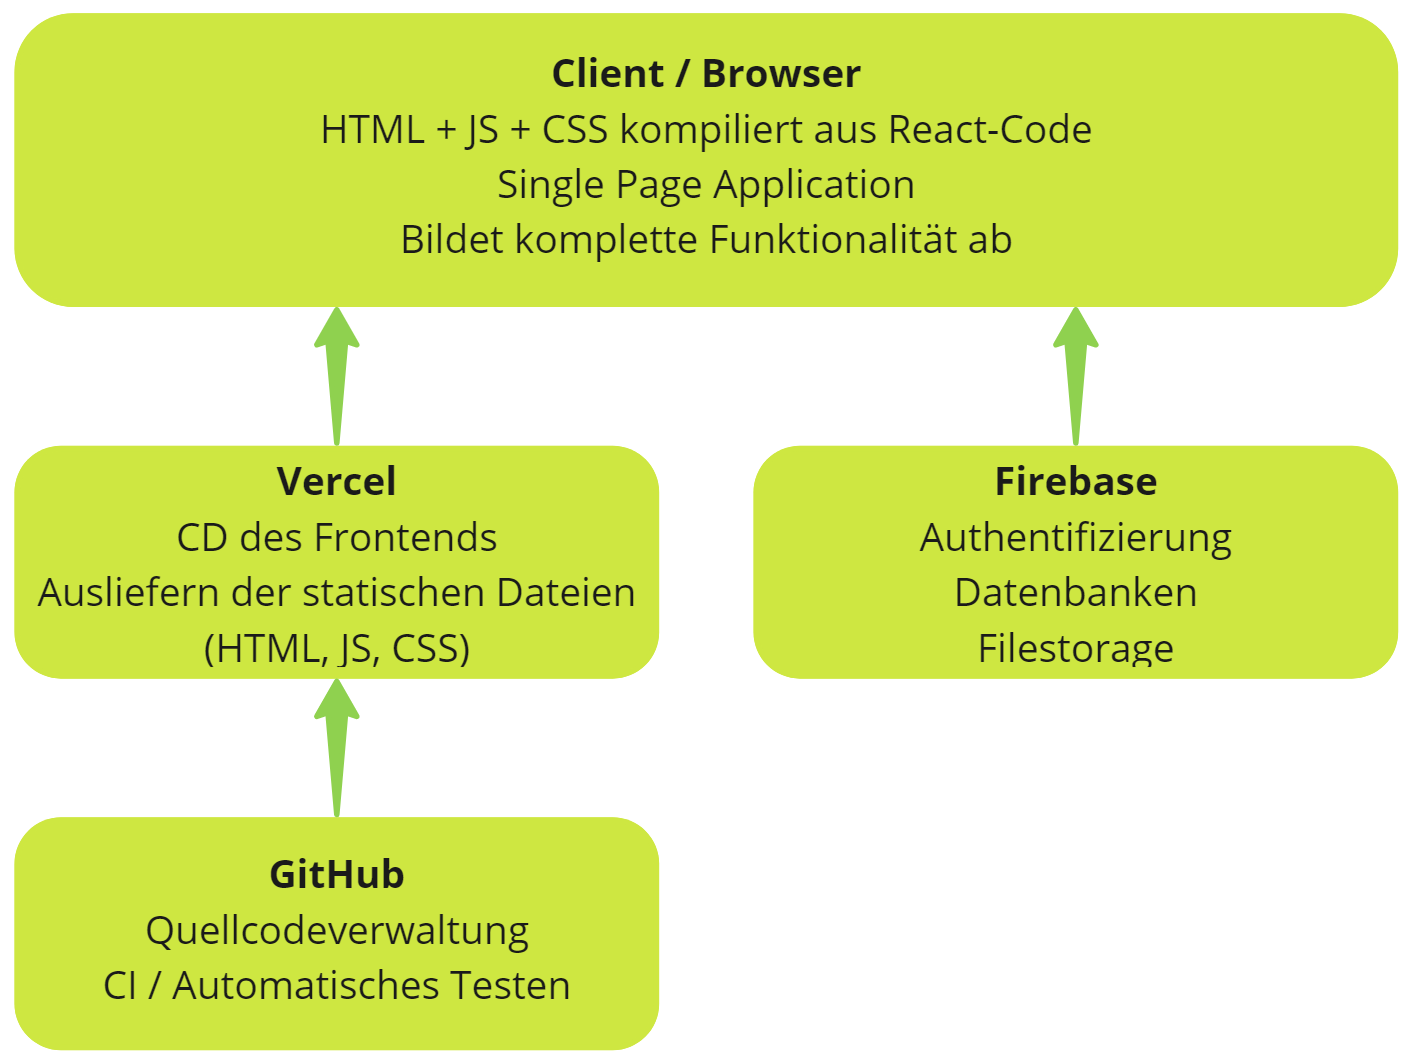
\includegraphics[width=.75\textwidth]{figures/architecture/architecture.png}
    \caption{Übersicht der technischen Softwarearchitektur}
    \label{fig:technicalArchitecture}
  \end{centering}
\end{figure}

Das Frontend wird in React entwickelt. Dieses enthält die Single Page Application (SPA) für die Benutzeroberfläche. Die gesamte Funktionalität wird in diesem Frontend implementiert.
Um im Team bei der Entwicklung effizient zusammenzuarbeiten, wir als Quellcodeverwaltungstool Git bzw. Github verwendet.
Wird eine Änderung am Quellcode veröffentlicht, werden automatisch die CI / CD Prozesse gestartet.
Sind die Tests erfolgreich, wird die neue Version über Vercel gehostet.

Wird der entsprechende Internetlink im Browser aufgerufen, erhält der anfragende Client (Browser) die statischen Dateien für die Benutzeroberfläche.
Der Browser führt das darin enthaltene Javascript aus, das ein dynamisches Laden der Inhalte der Datenbank (Firebase) ermöglicht.
